\red{Management and administration information:
•	Gantt chart (schedule) – Include important issues associated with task duration prediction – presented in your “Progress Reports”.
•	Cumulative hours spent on project – individual and/or team based, project diaries,
•	Individual or team based project diary.
}

\subsection{Gantt Chart}
\todomessage{Gantt Chart}

\subsection{Major Problems and Issues}
\begin{itemize}
	\item Vibrations and stability: In semester 1, more time than initially planned was spent on eliminating vibrations and increasing stability of the aircraft. 
	\item Printer repair: Many hours have been spent fixing and tweaking the 3D printer.  At one point over the holidays, a whole week of testing and repair was done to fix an issue with the nozzles. See gant chart xxx
	\item Many crashes: Crashes throughout the year required ordering more parts and waiting. It also required lots of fixing and debugging. Huge amounts of time spent of time had to be then spent re-testing. All major crashes were to do with faulty hardware such as the power module, RC receiver and transmitter and the motor failure. This meant the fixed wing flight controller could not be 100\% completed. See gant chart and flight tests xxx.
	\item Redundent Team Member: Shanon stopped contributing after semester 1. He was only there for meetings and presentations. Whole sections of the Gantt Chart are not complete as they were his responsibilities. see xxx
\end{itemize}
\todomessage{reference gantt}

\subsection{Project Diary}
The team has made extensive use of Trello to maintain records of the tasks performed throughout the project. The project's records/diary may be viewed in full detail here: \url{https://trello.com/uavoutbackchallenge2016}.

\todomessage{Cumulative hours}

\subsection{Flight Tests}
\label{sec:diary}

\begin{table}[!htbp]
	\centering
	\caption{Flight tests performed by \ID}
	\begin{tabular}{|c|c|c|c|c|c|c|}
		\hline Date & Location & Flight Time & Aim & Result & Problems \\ 
		\hline 13/05/15 & Melb Uni & 2 min & Courtyard Winged Hover test & Complete & - \\ 
		\hline 02/07/15 & Melb Uni & 2 min & Courtyard Alt-Hold test & Complete & - \\ 
		\hline 03/07/15 & Cardinia & 15 min & Major test/Autotune & Complete & Radio cut outs \\ 
		\hline 27/07/15 & Cardinia  & 0 min & Autotune new firmware & Incomplete & Radio faillure \\ 
		\hline 31/07/15 & Cardinia  & 6 min & Autotune new firmware & Crash & Motor burnt out, damage  \\ 
		\hline 22/08/15 & Cardinia  & 2 min & Autotune new firmware & Crash & Power Module Failure, damage\\
		\hline 04/09/15 & Melb Uni & 1 min & Courtyard Alt-Hold test & Complete & - \\  
		\hline 05/09/15 & Cardinia  & 8 min & Autotune new firmware & Complete & Back gear broken\\
		\hline 18/07/15 & Melb Uni & 1 min & Courtyard Alt-Hold test & Complete & - \\  
		\hline 19/09/15 & Cardinia  & 10 min & Test flight with wings & Complete & Overheating \\ 
		\hline 27/09/15 & Cardinia  & 5 min & Test transition & Incomplete & Solder melting (overheating) \\ 
		\hline 
	\end{tabular} 
	\label{tab:tests}
\end{table}

\subsection{Scope of Works}
See below for the final version of team \ID Scope of Works.
\includepdf[pages=2-]{scope.pdf}